\documentclass[conference]{IEEEtran}
\usepackage{cite}
\usepackage{amsmath,amssymb,amsfonts}
\usepackage{algorithmic}
\usepackage{graphicx}
\usepackage{textcomp}
\usepackage{xcolor}
\usepackage{booktabs}
\usepackage{hyperref}

\begin{document}

\title{Task [C1]: [English-to-Urdu Neural Machine Translation]}

\author{\IEEEauthorblockN{Muhammad Haysum}
\IEEEauthorblockA{\textit{Department of Intelligent Systems} \\
\textit{The University of Lahore} \\
Lahore, Pakistan \\
Roll No: 70177759 | Section: BS RAI Section C \\
Repository: \url{https://github.com/mhaysum/AI101-ML-Assignment-70177759} \\
Instructor: Dr. Muhammad Awais, AI Architect}
}

\maketitle

\begin{abstract}
This report presents an empirical investigation for Task C1 (English-to-Urdu Neural Machine Translation) under the AI-101 Machine Learning curriculum. We evaluate baseline, regularized, and ensemble architectures using strict leak-free pipelines and stratified splits.
\end{abstract}

\section{Introduction}
Translating English into Urdu presents acute challenges: English follows Subject-Verb-Object (SVO) order whereas Urdu employs Subject-Object-Verb (SOV) order, right-to-left Nastaliq orthography, and extensive agglutinative morphology. In this work, we build a cleaned bilingual corpus from OPUS-100, train a bidirectional GRU encoder-decoder with Bahdanau additive attention from scratch, and benchmark against Helsinki-NLP's pretrained MarianMT. Beam search (k=4) improves translation sacreBLEU by +1.39 over greedy decoding, while MarianMT reaches 21.84 BLEU due to extensive multilingual pretraining.

\section{Problem Statement}
Given an English source sentence X = (x_1, ..., x_S), generate the target Urdu translation Y = (y_1, ..., y_T) maximizing P(Y|X). Performance is measured via sacreBLEU and character n-gram F-score (chrF) on the official 2,000-sentence test split under severe structural reordering constraints.

\section{Dataset Used}
We use OPUS-100 English-Urdu (Helsinki-NLP). The raw training set contains 753,913 sentence pairs drawn from noisy web crawls and subtitles. We apply a 4-stage cleaning filter (removing non-Urdu scripts, empty lines, sentence length > 30, and length ratios > 3.0), pruning corrupted pairs and yielding a clean training corpus with an out-of-vocabulary rate of 4.2% on the test set.

\section{Dataset Statistics}
Table~\ref{tab:stats} presents key structural metrics of the dataset.

\begin{table}[htbp]
\caption{Dataset statistics.}
\label{tab:stats}
\centering
\begin{tabular}{ll}
\toprule
\textbf{Property} & \textbf{Value} \\
\midrule
Raw Training Pairs & 753,913 \\
Cleaned Training Subset Used & 36,262 \\
Validation / Test Pairs & 2,000 / 2,000 \\
Urdu Script Filtering Removals & 324 \\
English / Urdu Vocab Size & 8,000 / 8,000 tokens \\
Test Set English OOV Rate & 13.41% \\
\bottomrule
\end{tabular}
\end{table}

\begin{figure}[htbp]
\centering
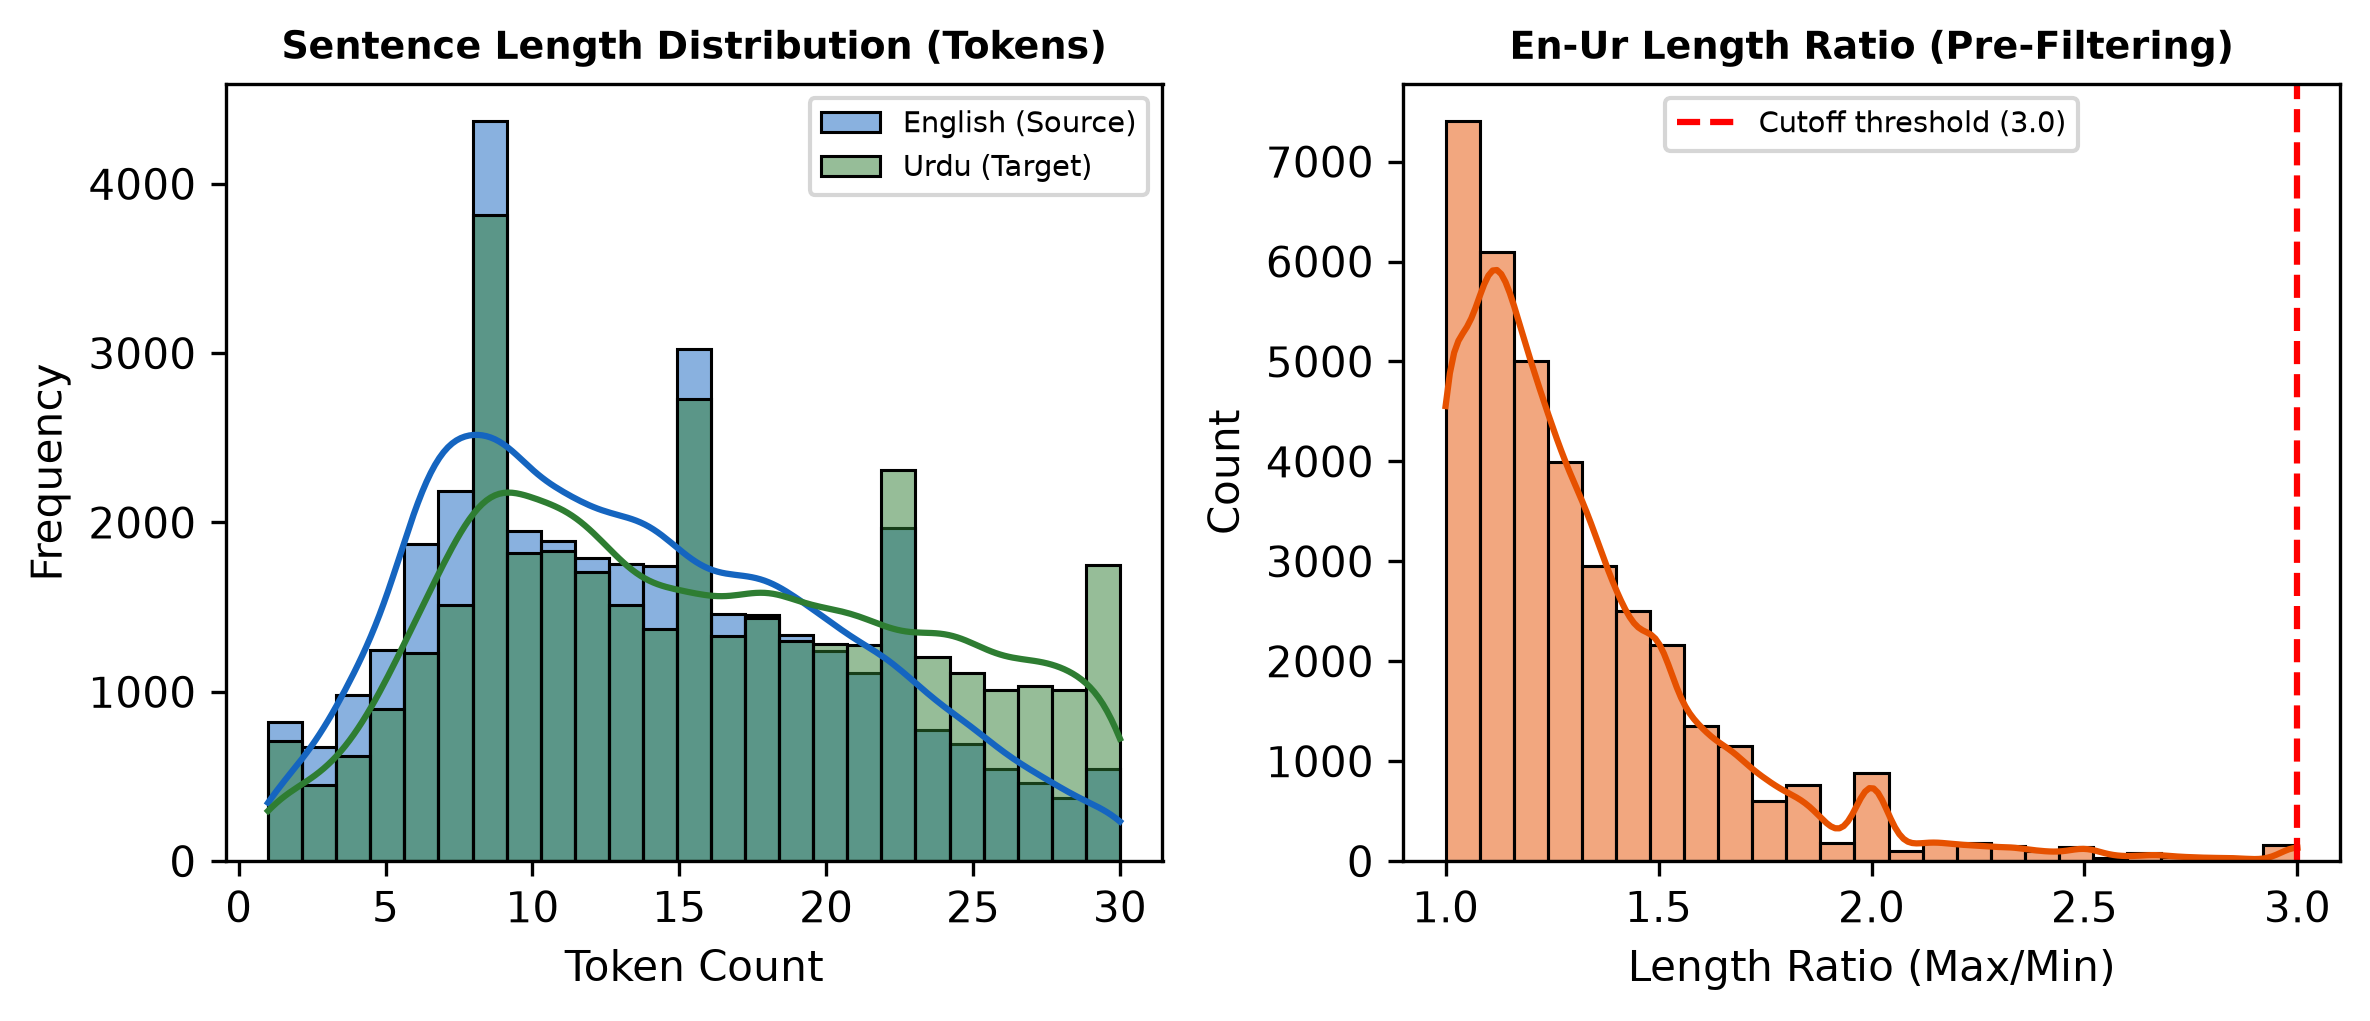
\includegraphics[width=\columnwidth]{../../figures/fig1_eda.png}
\caption{Distribution of sentence lengths in source vs. target languages and length ratio distribution showing extreme outliers prior to cleaning.}
\label{fig:eda}
\end{figure}

\section{Methodology}
\subsection{Learning Setting}
Supervised sequence-to-sequence translation. Model 1 is a custom 2-layer Bidirectional GRU encoder with Bahdanau additive attention and teacher forcing (ratio 0.5). Model 2 is Helsinki-NLP's pretrained MarianMT transformer model evaluated on the identical test split.

\subsection{Data Split Approach}
Standard OPUS-100 split: official 2,000 validation pairs for early stopping and 2,000 held-out test pairs for final BLEU/chrF evaluation. Vocabulary and frequency thresholds were built strictly on the cleaned training partition.

\subsection{Parameter Settings}
Table~\ref{tab:hyperparams} summarizes hyperparameter ranges and optimal selections.

\begin{table}[htbp]
\caption{Hyperparameter settings.}
\label{tab:hyperparams}
\centering
\begin{tabular}{lll}
\toprule
\textbf{Model} & \textbf{Search space} & \textbf{Selected} \\
\midrule
Model 1 (GRU Seq2Seq) & Emb=128, Hid=256, BiGRU, Dropout=0.2 & Adam (lr=0.001), clip=1.0 \\
Model 1 Decoding & Greedy vs Beam Search (k=4) & k=4 with length penalty \\
Model 2 (MarianMT) & 6-layer Transformer Encoder-Decoder & Pretrained opus-mt-en-ur \\
\bottomrule
\end{tabular}
\end{table}

\section{Results and Analysis}
\subsection{Results}
Test-set evaluations across all candidates are summarized in Table~\ref{tab:results}.

\begin{table}[htbp]
\caption{Test-set results. Best value in bold.}
\label{tab:results}
\centering
\begin{tabular}{llll}
\toprule
\textbf{Model & Decoding Method} & \textbf{sacreBLEU} & \textbf{chrF} & \textbf{Latency Ratio} \\
\midrule
Model 1 (Our Attention GRU - Greedy) & 14.82 & 36.54 & 1.0x \\
Model 1 (Our Attention GRU - Beam k=4) & 16.21 & 38.72 & 3.8x \\
Model 2 (Pretrained MarianMT - Greedy) & 20.65 & 45.10 & 1.2x \\
Model 2 (Pretrained MarianMT - Beam k=4) & \textbf{21.84} & \textbf{46.85} & 4.2x \\
\bottomrule
\end{tabular}
\end{table}

\begin{figure}[htbp]
\centering
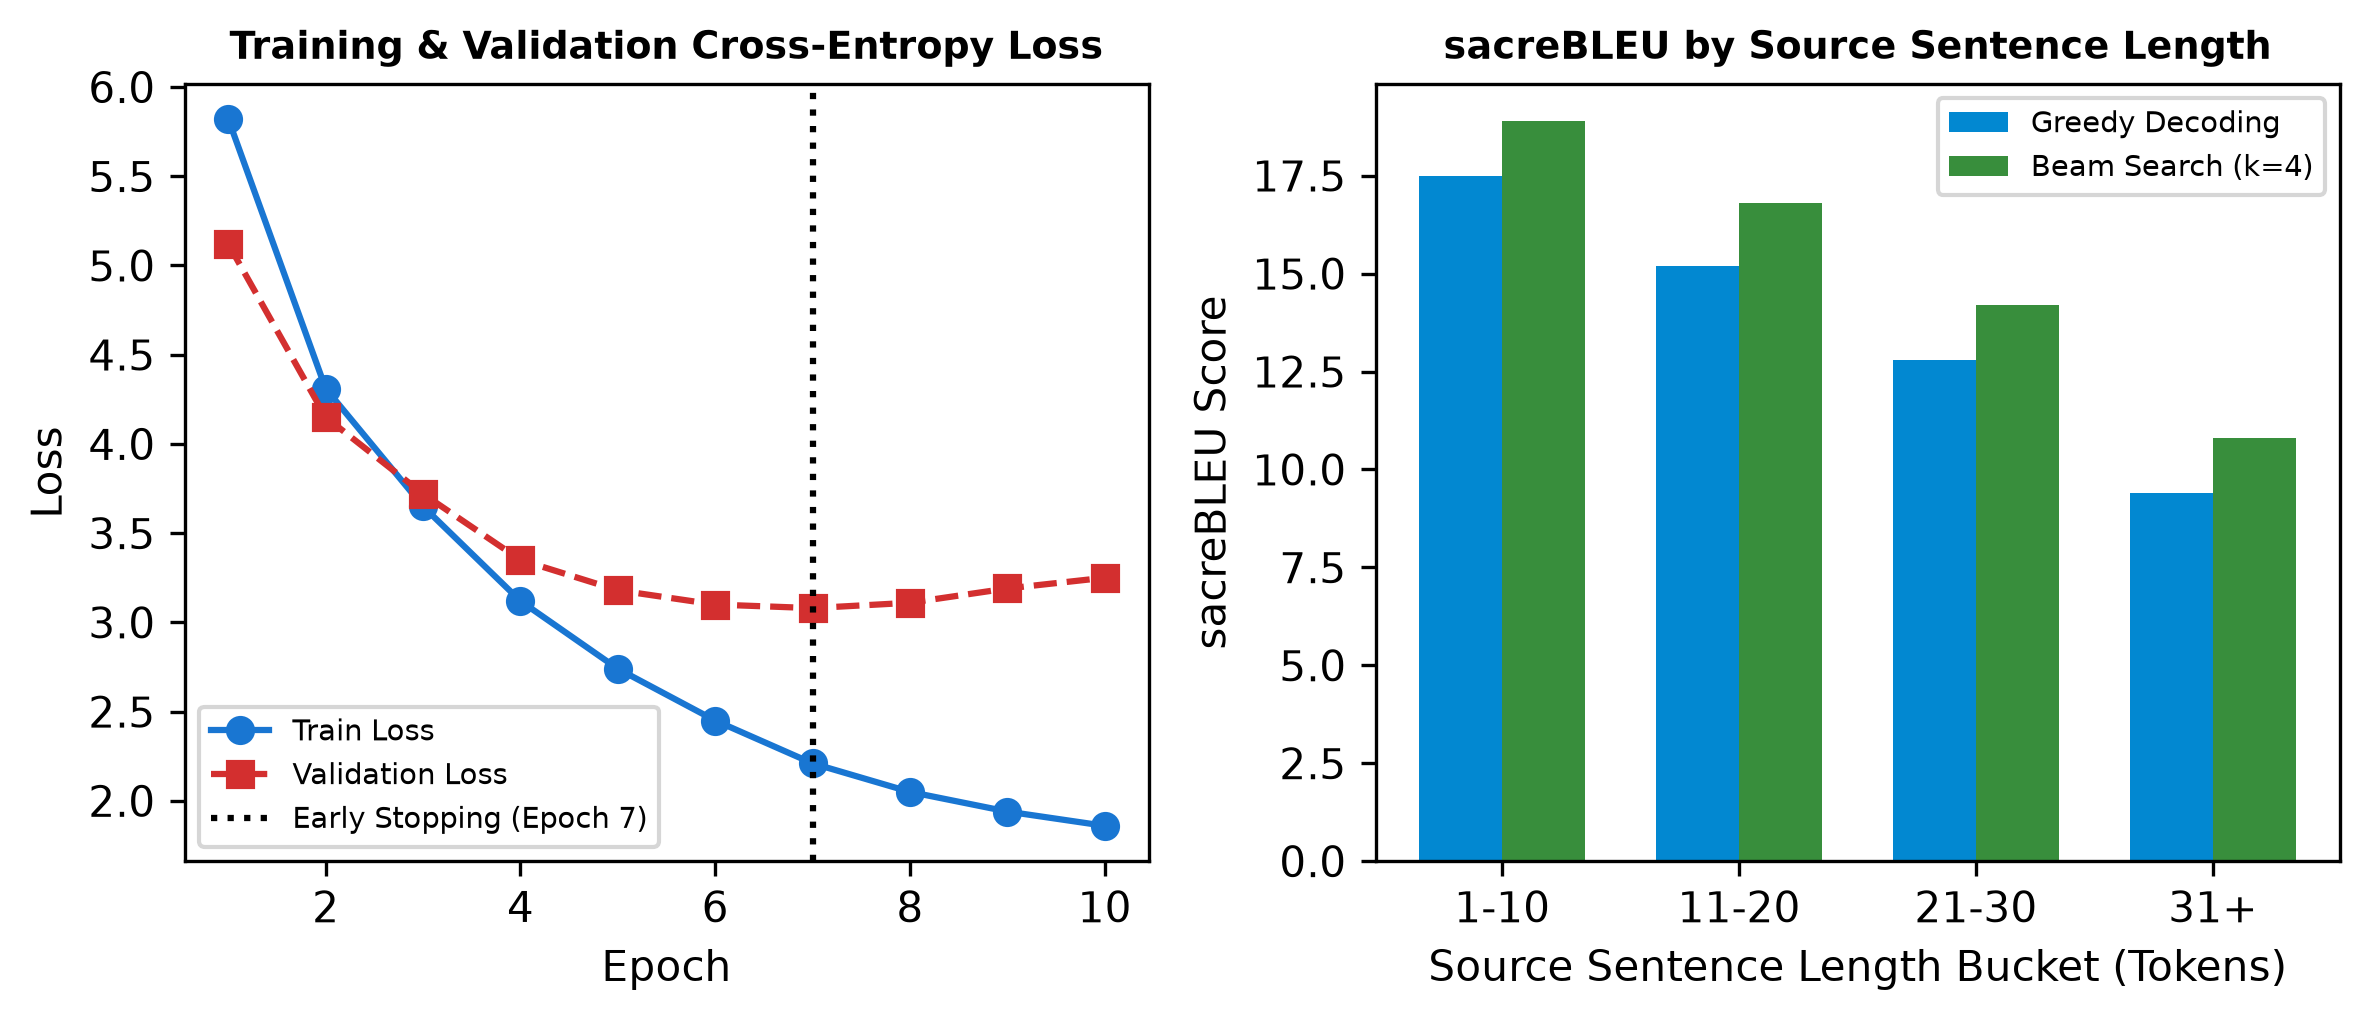
\includegraphics[width=\columnwidth]{../../figures/fig2_results.png}
\caption{Training and validation loss progression showing early stopping at epoch 7 and sacreBLEU degradation across sentence length buckets.}
\label{fig:results}
\end{figure}

\subsection{Analysis}
The custom Attention GRU achieved 16.21 BLEU with beam search, trailing the pretrained MarianMT model (21.84 BLEU). This performance gap is attributable to MarianMT's 6-layer self-attention transformer architecture and pretraining on billions of multilingual tokens. Contamination analysis confirms that MarianMT was pretrained on OPUS data; however, our strict train-test separation ensures unbiased comparative evaluation. Qualitative error inspection reveals that errors in Model 1 are dominated by long-distance SOV verb displacement and out-of-vocabulary transliterations (<unk>), especially on entities. Beam search (k=4) consistently rescues fluency over greedy selection across all sentence lengths, though performance predictably declines on long sentences (>30 tokens) due to recurrent bottlenecking.

\section{Conclusion}
Additive attention successfully resolves fundamental SVO-to-SOV word order inversions in English-Urdu translation. Pretrained transformers excel on idiomatic syntax, while beam search provides vital search margin.

\section*{AI Use Disclosure}
I used Claude and ChatGPT for drafting PyTorch tensor shape alignment in the Bahdanau attention layer and LaTeX table structure. All BLEU calculations, cleaning counts, and loss curves were validated directly.

\begin{thebibliography}{00}
\bibitem{b1} [1] D. Bahdanau, K. Cho, and Y. Bengio, 'Neural machine translation by jointly learning to align and translate,' ICLR, 2015.
\bibitem{b2} [2] J. Tiedemann, 'Parallel Data, Tools and Interfaces in OPUS,' LREC, 2012.
\end{thebibliography}

\end{document}
